\section{Konzeption}

Dieses Kapitel entwickelt die Konzeption des Prototyps auf Grundlage der zuvor formulierten Anforderungen sowie der technischen Randbedingungen von eBPF.
Zunächst werden die praktischen Einschränkungen der Ausführung im Kernelspace eingeordnet.
Darauf aufbauend werden die Architektur mit ihren Zuständigkeiten, die Datenflüsse und das fachliche Datenmodell beschrieben.
Abschließend werden die wesentlichen Entwurfsentscheidungen, ihre Alternativen und ihre jeweiligen Konsequenzen begründet.



\subsection{Entwurfsfolgen der eBPF-Einschränkungen}
Die in Abschnitt~\ref{sec:ebpf-verifier} beschriebenen Grenzen erfordern für den Prototyp feste Datenlayouts, begrenzte Schleifen und eine überschaubare Auswertungslogik. Daraus folgen drei Entwurfsentscheidungen: Textuelle Policies werden im Userspace vorbereitet, der Kernel erhält kompakte Regeln und Attribute über Maps, und die Auswertung wird auf mehrere Tail-Call-Stufen verteilt. Die jeweiligen Begründungen folgen in den Entwurfsentscheidungen dieses Kapitels.

\subsection{Architektur}

Die Architektur des Prototyps ist in zwei zentrale Bereiche unterteilt: den Userspace und den Kernelspace. 
Die Gründe für diese Aufteilung werden in Abschnitt~\ref{sec:entscheidung-userspace-kernelspace} erläutert.
Die im Folgenden verwendeten Bezeichnungen Kernelspace-PEP und Userspace-PEP heben die jeweilige Durchsetzungsfunktion hervor.
Wie in den Grundlagen erläutert, enthalten beide Pfade zugleich eine integrierte PDP-Funktion, weil sie die anwendbaren Policies lokal auswerten und daraus eine Entscheidung ableiten.
Ein separater PDP-Prozess und ein Nachrichtenaustausch von Entscheidungsanfragen und Entscheidungen zwischen PDP und PEP sind nicht Bestandteil der Architektur.

Die Zuständigkeiten verteilen sich auf folgende Komponenten:
\begin{description}
    \item[Hauptprogramm:] Initialisiert Maps und eBPF-Programme, hängt den LSM-Hook an und steuert die Userspace-Komponenten.
    \item[Policyverwaltung:] Liest und validiert Policyquellen, übersetzt sie in Regeln und aktiviert neue Policy-Generationen.
    \item[Attributloader:] Stellt die aktuelle Zeit sowie externe System-, Subject- und Ressourcenattribute bereit.
    \item[Kernelspace-PEP:] Bewertet neue Dateiöffnungen am Hook \texttt{file\_open} und setzt die Entscheidung über dessen Rückgabewert durch.
    \item[Userspace-PEP:] Rekonstruiert nach entscheidungsrelevanten Ereignissen bestehende Dateizugriffe und versucht, unzulässige FDs gezielt zu schließen.
    \item[Administrationstool:] Zeigt geladene Policies, Attribute und Generationen ausschließlich lesend an.
\end{description}

Gepinnte eBPF-Maps verbinden die Komponenten durch gemeinsame Entscheidungsdaten. Entscheidungen verbleiben im jeweiligen Durchsetzungspfad; der Userspace-PEP erhält keine fertigen Entscheidungen vom Kernel, sondern bewertet bestehende Zugriffe selbst. Die Zuordnung dieser Aufgaben zu Rust-Crates behandelt Abschnitt~\ref{sec:implementierungsstruktur}.

\begin{figure}[ht]
    \centering
    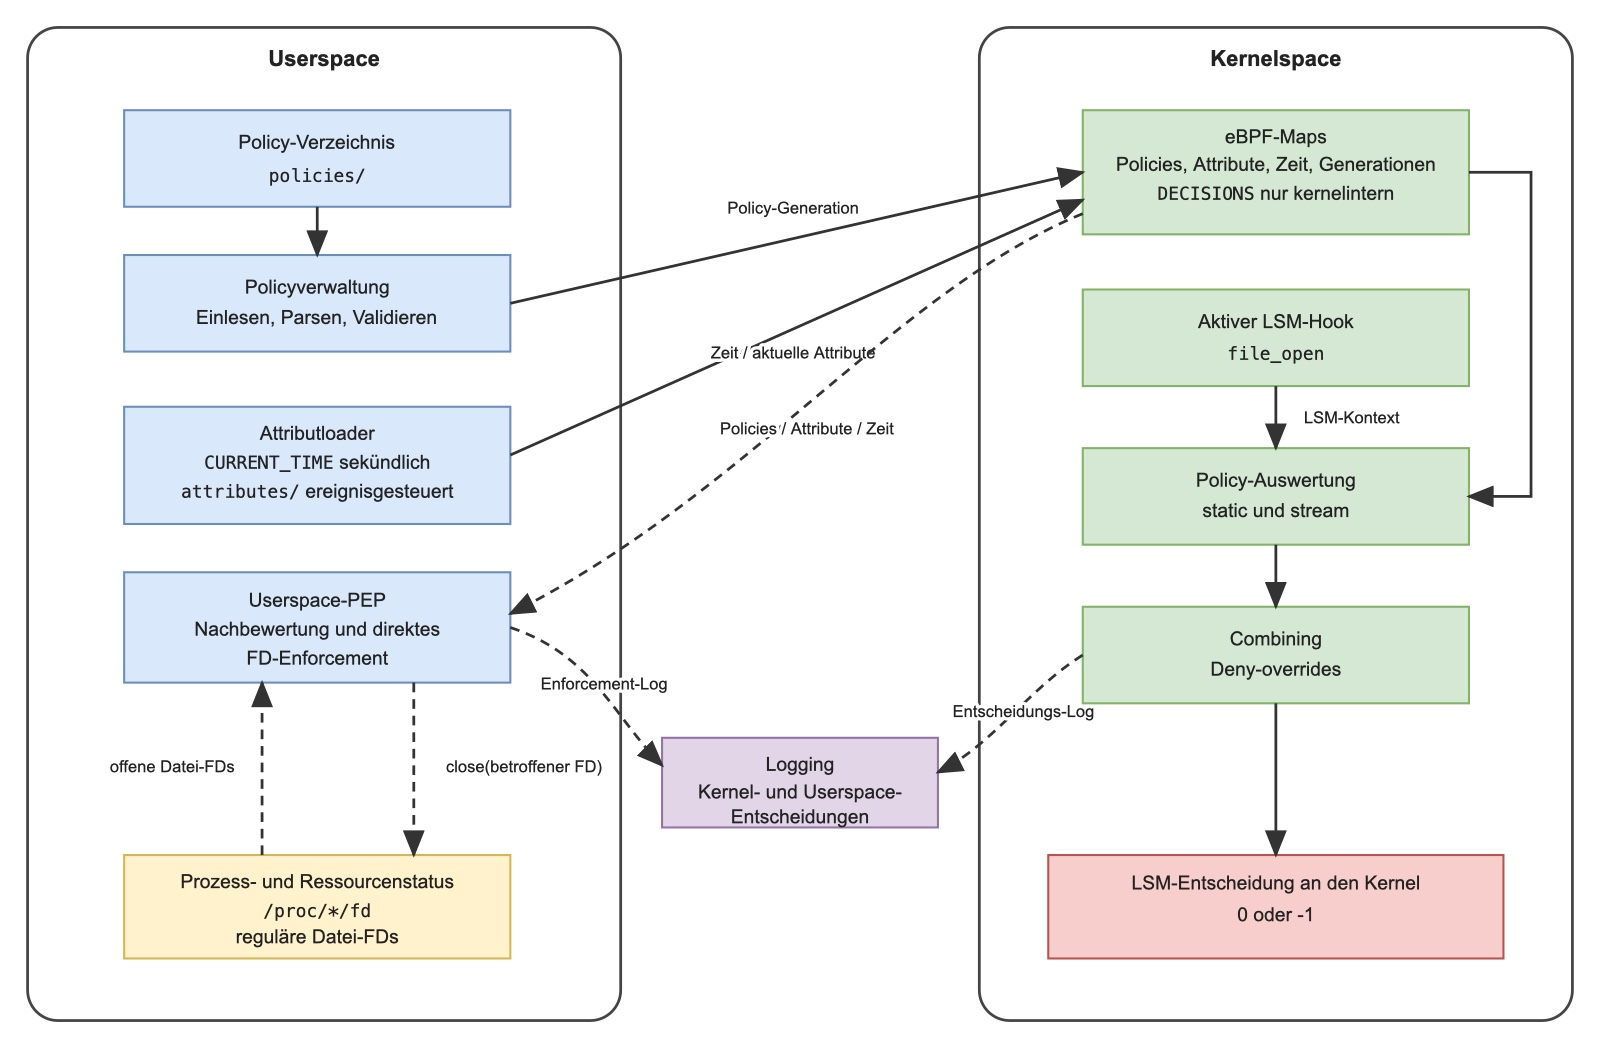
\includegraphics[width=0.95\textwidth]{graphics/architecture}
    \caption{Konzeptionelle Architektur des Prototyps}
    \label{fig:konzeption-architektur}
\end{figure}


\subsection{Datenfluss}
Die vier Abläufe verbinden die Eingabedaten mit der unmittelbaren und nachträglichen Zugriffskontrolle.

\subsubsection{Policy-Datenfluss}
Die Policyverwaltung liest den veröffentlichten Dateibestand, validiert ihn und erzeugt kernelgeeignete Regeln. Erst nach erfolgreicher Vorbereitung wird die neue Policy-Generation aktiviert; Updatefehler vor der Aktivierung lassen die bisherige Generation bestehen. Das Generationenmodell und seine Grenzen erläutert Abschnitt~\ref{sec:entscheidung-policy-generationen}.

\subsubsection{Datenfluss dynamischer Attribute}
Die aktuelle Zeit wird regelmäßig bereitgestellt, externe Attribute nach Veröffentlichung oder Entfernung aktiver Quelldateien. Das Veröffentlichungsprinzip ist die atomare Ersetzung einer vollständig vorbereiteten Datei; es bildet keine gemeinsame Transaktion mehrerer Dateien oder einen atomaren Verzeichnissnapshot. Das konkrete Verfahren beschreibt Abschnitt~\ref{sec:konfigurationsveroeffentlichung}. Nach erfolgreicher Verarbeitung wird der neue Attributbestand unabhängig von den Policies aktiviert.

\subsubsection{Zugriffsentscheidungen im Kernel}
Der Hook \texttt{file\_open} liefert den Kontext einer neuen Dateiöffnung. Der Kernelspace-PEP bildet daraus eine Anfrage, prüft die geladenen Regeln und kombiniert deren Ergebnisse. Bei einer Ablehnung unterbindet der Kernel die Öffnung. Die gewählte Combining-Semantik erläutert Abschnitt~\ref{sec:combining-konzept}.

\subsubsection{Nachträgliche Kontrolle bestehender Zugriffe}
Eine erfolgreiche entscheidungsrelevante Aktivierung oder eine relevante Zeitgrenze löst die Nachbewertung bestehender FDs aus. Der Userspace-PEP rekonstruiert diese Zugriffe aus Betriebssysteminformationen, wertet die gepinnten Entscheidungsdaten aus und versucht, betroffene FDs zu schließen. Begründung und Best-Effort-Grenzen stehen in Abschnitt~\ref{sec:nachbewertung-konzept}.

\subsection{Fachliches Datenmodell}
Das Datenmodell unterscheidet Eingaben, vorbereitete Entscheidungsgrundlagen und eine konkrete Auswertung:
\begin{description}
    \item[Policyquelle:] Eine menschenlesbare Datei beschreibt Entscheidung, Zugriffstyp, Filter und Bedingungen.
    \item[Vorbereitete Regeln:] Validierte Policyquellen werden in statische Regeln und Streampolicies übersetzt. Eine Policy-Generation umfasst die gemeinsam aktivierte Regelmenge.
    \item[Attribute:] Zeitinformationen und externe Werte beschreiben den veränderlichen Kontext. Externe Attribute gehören zum System, zu einem Subjekt oder zu einer Ressource und besitzen eine eigene Generation.
    \item[Zugriffsanfrage:] Subjekt, Kommando und Dateiobjekt beschreiben eine neue Öffnung oder einen rekonstruierten bestehenden Zugriff. Für den nachträglichen Entzug kommen Prozess-ID und FD-Nummer hinzu.
    \item[Entscheidungszustand:] Treffer der Regelauswertung werden als Permit- und Deny-Markierungen gesammelt und zu einer Gesamtentscheidung kombiniert.
\end{description}
Die konkreten Structs, Feldgrößen und Map-Typen dieser Objekte beschreibt Abschnitt~\ref{sec:map-abi}.

\subsection{Entwurfsentscheidungen}

Die folgenden Entwurfsentscheidungen leiten aus den fachlichen Anforderungen und den technischen
Rahmenbedingungen die grundlegende Gestaltung des Prototyps ab. Für jede Entscheidung werden das
Ausgangsproblem, die gewählte Lösung, berücksichtigte Alternativen und die daraus entstehenden
Konsequenzen dargestellt.

\subsubsection{Policy-Verarbeitung im Userspace und Auswertung im Kernelspace}\label{sec:entscheidung-userspace-kernelspace}
Das Reference-Monitor-Konzept verlangt eine manipulationssichere, verifizierbare Komponente zur Überprüfung der Zugriffe auf geschützte Ressourcen \cite[Abschnitt~3.4]{anderson1972computer}. LSM-Hooks erlauben die Entscheidung unmittelbar im Kernel-Ausführungspfad \citep{wright2002linux}. Der Prototyp trifft daher die Entscheidung über eine neue Öffnung im Kernel, bereitet ihre Eingabedaten aber im Userspace vor.

Textuelles Parsen und Validieren benötigt Zeichenkettenverarbeitung, Zwischendaten und aussagekräftige Fehlerbehandlung. Eine solche Verarbeitung im eBPF-Programm würde dessen begrenzten Stack und die Verifier-Prüfung belasten. Gewählt wird deshalb eine Userspace-Verarbeitung, die lesbare Policydateien in feste Regeln mit Subjekt-, Kommando-, Ressourcen- und Bedingungsfeldern übersetzt. Der Kernel beschränkt sich auf Vergleiche, Map-Lookups und begrenzte Schleifen. Dies hält den unmittelbaren Durchsetzungspfad klein und nachvollziehbar.

Eine Alternative wäre das direkte Schreiben binärer Regeln in Maps, etwa mit \texttt{bpftool}. Dabei müssten Nutzer Layout und Validierung selbst sicherstellen; ganze Policy-Stände wären schwerer nachvollziehbar auszutauschen. Eine mächtigere Policy-Engine im Kernel würde mehr Ausdrucksstärke bieten, aber die eBPF-Grenzen stärker belasten. Eine Beschränkung auf rein statische Regeln würde dagegen die für ASBAC wesentlichen dynamischen Bedingungen auslassen.

Die gewählte Trennung erhält die nutzerseitige Policybeschreibung und begrenzt zugleich das unterstützte Kernelmodell. Erweiterungen müssen in dessen feste Repräsentation passen oder zusätzliche Vorverarbeitung erhalten. Der Userspace übernimmt außerdem die Attributbereitstellung und die nachträgliche Kontrolle bestehender Zugriffe; die unmittelbare Öffnungsentscheidung bleibt im Kernel.

\subsubsection{Einsatz von eBPF-LSM statt eines klassischen LSM}
Klassische LSM werden im Mainline-Linux in den Kernel eingebaut und können nicht wie gewöhnliche Kernelmodule zur Laufzeit nachgeladen werden~\cite{kernelorgLSM}.
Änderungen an ihrer Implementierung erfordern daher üblicherweise einen erneuten Kernelbuild und den Start des angepassten Kernels.
Davon zu unterscheiden sind Änderungen an den Policies eines bestehenden LSM, etwa SELinux, die keinen erneuten Kernelbuild erfordern.
Für den experimentellen Prototyp ist insbesondere die Möglichkeit relevant, den eigenen Zugriffskontrollcode ohne erneuten Kernelbuild zu ändern.

Gewählt wurde daher die Implementierung als eBPF-LSM.
Diese Implementierung erlaubt es, eBPF-Programme an LSM-Hooks auszuführen und damit Zugriffskontrollentscheidungen im Kernel-Ausführungspfad zu treffen~\cite{kernelBpfLsm}.
Bei einem entsprechend konfigurierten Kernel mit aktiviertem BPF-LSM können die Programme zur Laufzeit geladen und an unterstützte LSM-Hooks angehängt werden; vor der Ausführung werden sie durch den eBPF-Verifier geprüft~\cite{kernelBpfLsm,kernelBpfVerifier}.

Ein weiterer Grund für diese Entscheidung ist die Möglichkeit, eBPF-Programme mit Rust zu entwickeln.
Der Prototyp nutzt dafür Aya (siehe Abschnitt~\ref{sec:aya}).
Dadurch können Userspace- und eBPF-Anteile innerhalb desselben Rust-Workspaces entwickelt werden.
Zusätzlich können gemeinsame Datenstrukturen und Teile der Policy-Auswertungslogik in einer
gemeinsamen Rust-Kompilationseinheit (Crate) abgebildet werden.
Dies verbessert die Konsistenz zwischen Userspace und Kernelspace und reduziert doppelte Implementierungen.

Eine Alternative wäre die Entwicklung eines klassischen LSM gewesen.
Diese Alternative bietet grundsätzlich größere Freiheiten im Kernelcode, erhöht jedoch Entwicklungs- und Wartungsaufwand.
Für den Prototyp ist eBPF-LSM geeigneter, da Änderungen schneller getestet werden können und gleichzeitig ein sicherheitsrelevanter Ausführungspunkt im Kernel genutzt wird.

Konsequenzen dieser Entscheidung sind, dass die Implementierung die Einschränkungen von eBPF beachten muss, insbesondere die Prüfung durch den Verifier, die begrenzte Stack-Nutzung und die eingeschränkte Programmkomplexität.
Diese Einschränkungen beeinflussen unter anderem die Aufteilung der eBPF-Programme in verschiedene Tail-Calls und die reduzierte Policy-Repräsentation im Kernelspace.


\subsubsection{Auswahl des LSM-Hooks}
Für den Prototyp musste ein LSM-Hook ausgewählt werden, an dem sich die unmittelbare Zugriffskontrolle und die spätere Überwachung bestehender Zugriffssituationen nachvollziehbar untersuchen lassen.
Die Wahl fiel auf den Hook \texttt{file\_open}.
Dieser Hook wird im regulären Öffnungspfad über \texttt{security\_file\_open} aufgerufen und passt damit unmittelbar zu der Anforderung, Dateiöffnungen zu kontrollieren.
Eine ablehnende Entscheidung bricht den Öffnungsvorgang ab, sodass dem aufrufenden Prozess kein FD für diese Öffnung zurückgegeben wird.
Für den aufrufenden Prozess liefert \texttt{open} bei einer Ablehnung \texttt{-1} statt eines neuen FDs zurück~\citep{linuxFileOpenSource,linuxFileSecuritySource,manOpen}.

Eine unmittelbare Alternative für die Kontrolle von Dateizugriffen ist der Hook \texttt{file\_permission}.
Dieser wird über \texttt{security\_file\_permission} vor Lese- und Schreiboperationen auf einer bereits geöffneten Datei aufgerufen und ermöglicht insbesondere eine erneute Rechteprüfung nach Policy-Änderungen~\citep{linuxFileSecuritySource}.
Würde die Policy ausschließlich an diesem Hook durchgesetzt, könnte die reguläre Dateiöffnung zunächst erfolgreich sein und einen FD zurückgeben, sofern die übrigen Berechtigungsprüfungen den Vorgang erlauben.
Eine ablehnende Entscheidung würde dann die nachfolgende, vom Hook erfasste Lese- oder Schreiboperation verhindern; der bereits geöffnete FD würde dadurch nicht geschlossen~\citep{linuxFileOpenSource,linuxFileReadWriteSource}.
Der Unterschied liegt somit zwischen der Verhinderung einer erfolgreichen Dateiöffnung und der erneuten Autorisierung einzelner Operationen über einen bestehenden FD.

Für den Prototyp wird \texttt{file\_open} gewählt, weil bereits der Aufbau der betrachteten Zugriffssituation verhindert werden soll, wenn die Policy ihn nicht erlaubt.
Nach einer erlaubten Öffnung kann der entstandene FD dagegen als Ansatzpunkt für die spätere Überwachung dienen.
Wird seine weitere Nutzung durch eine Policy- oder Attributänderung unzulässig, veranlasst der Userspace-PEP das Schließen des betroffenen FDs.
Bei erfolgreichem Schließen steht diese Referenz auf die Datei für neue Operationen nicht mehr zur Verfügung~\citep{manClose}.
Damit werden die anfängliche Zulassung im Kernel und der nachträgliche Entzug im Userspace an derselben, über einen FD repräsentierten Zugriffssituation untersucht.
Diese Aufteilung ersetzt keine synchrone Policy-Prüfung vor jeder Lese- oder Schreiboperation: Zwischen einer Änderung und dem nachträglichen Schließen verbleibt ein Zeitfenster.

Dateiöffnungen und fortdauernde FDs lassen sich mit Linux-Bordmitteln sowie \path{/proc/<PID>/fd} reproduzierbar beobachten \citep{manProcPidFd}. Netzwerkhooks wie \texttt{socket\_bind} würden einen anderen Zugriffstyp und zusätzliche Zustandsbeobachtung erfordern, ohne die hier untersuchte Fragestellung besser abzudecken.

Die Konsequenz dieser Entscheidung ist eine bewusste Begrenzung des Prototyps auf Dateiöffnungen.
Der Prototyp trifft damit keine allgemeine Aussage über alle möglichen LSM-Hooks, sondern untersucht ASBAC exemplarisch anhand eines gut beobachtbaren und reproduzierbar testbaren Zugriffstyps.



\subsubsection{Kommunikation über eBPF-Maps}
Der Prototyp benötigt eine gemeinsame Datenbasis zwischen Userspace und Kernelspace.
Der Userspace muss Policies, Attribute, Zeitinformationen und Generationenstände bereitstellen können.
Das eBPF-Programm muss diese Daten im LSM-Hook lesen können, ohne direkt auf Userspace-Speicher oder komplexe Userspace-Datenstrukturen zuzugreifen.
Zusätzlich müssen weitere Userspace-Komponenten, insbesondere Userspace-PEP und Administrationswerkzeug, den aktuellen Zustand lesen können.

Die Entscheidung lautet daher, die Kommunikation über eBPF-Maps umzusetzen.
Policy-Einträge werden in Array-Maps abgelegt, dynamische Attribute in der Hash-Map
\texttt{ATTRIBUTES}; \texttt{ATTRIBUTE\_GENERATION} kennzeichnet den aktiven Attributstand. Die gemeinsame
Zeitbasis liegt als Unix-Zeit in der einzigen Zeit-Map \texttt{CURRENT\_TIME}. Der gemeinsame Typ
\texttt{PolicyTime} leitet daraus für Kernelspace-PEP und Userspace-PEP identisch die benötigten
UTC-Komponenten ab.
Für Zustände, die über mehrere Komponenten hinweg zugreifbar sein müssen, werden gepinnte Maps verwendet.
Dadurch erhalten Loader, Userspace-PEP und Administrationswerkzeug einen stabilen Zugriffspfad auf dieselben Kernelobjekte, während das eBPF-Programm die Werte direkt im Kernel auswerten kann.
Die Map \texttt{DECISIONS} ist davon ausgenommen: Sie ist nicht gepinnt und speichert nur
Zwischenergebnisse zwischen den Tail-Call-Stufen des Kernelspace-PEP. Diese Entscheidungen werden
nicht in den Userspace übertragen, sondern erscheinen ausschließlich in den jeweiligen Logs.

Diese Entscheidung folgt aus dem eBPF-Ausführungsmodell.
eBPF-Programme können nicht beliebige Speicherbereiche des Userspace lesen und sollen im Zugriffspfad mit festen, vom Verifier nachvollziehbaren Datenstrukturen arbeiten.
eBPF-Maps sind der dafür vorgesehene Mechanismus, um Daten zwischen Userspace und eBPF-Programmen auszutauschen.
Sie ermöglichen es, Policy- und Attributzustände im Kernel bereitzustellen und dennoch aus dem Userspace heraus zu aktualisieren.
Zugleich passen Maps zu der reduzierten Policy-Repräsentation, weil sie feste Schlüssel- und Werttypen erzwingen.

Eine gleichwertige Alternative gibt es im Rahmen dieses Prototyps nicht.
Direkte Übergaben über Funktionsparameter sind für dauerhafte Policy- und Attributzustände nicht geeignet, weil der LSM-Hook bei jedem Zugriff unabhängig ausgeführt wird.
Ein erneutes Laden des eBPF-Programms bei jeder Policy- oder Attributänderung wäre unpraktisch und würde den laufenden Betrieb unnötig stören.
Userspace-Dateien können vom eBPF-Programm ebenfalls nicht als normale Dateien gelesen und interpretiert werden.
Damit bleiben eBPF-Maps die naheliegende und technisch vorgesehene Schnittstelle.

Die Konsequenz ist, dass alle zwischen Userspace und Kernel geteilten Zustände in feste Map-Layouts übersetzt werden müssen.
Änderungen an diesen Layouts betreffen beide Seiten und müssen deshalb kontrolliert erfolgen.
Gleichzeitig entsteht dadurch eine klare Schnittstelle: Der Userspace schreibt validierte Zustände in Maps, der Kernel liest diese Zustände bei der Zugriffskontrolle, und externe Komponenten können über gepinnte Maps lesend auf denselben Zustand zugreifen.

\subsubsection{Generationenmodell für Policy-Aktualisierungen}\label{sec:entscheidung-policy-generationen}
Policies können während des Betriebs geändert, hinzugefügt oder entfernt werden.
Dabei soll eine neue Policy-Generation erst nach vollständiger Vorbereitung zur Auswertung ausgewählt werden können.
Problematisch wäre beispielsweise, wenn einzelne Map-Einträge bereits überschrieben wurden, andere Einträge derselben Policy-Menge aber noch zum vorherigen Stand gehören.
In diesem Fall könnte eine Zugriffsentscheidung auf einer widersprüchlichen Mischung aus Einträgen der bisherigen und der neu vorbereiteten Policy-Generation beruhen.

Die Entscheidung lautet daher, Policy-Aktualisierungen über ein Generationenmodell umzusetzen.
Als Bank wird im Folgenden einer von zwei logisch getrennten Speicherbereichen innerhalb derselben
Map bezeichnet. Eine Bank ist somit weder ein eigener eBPF-Map-Typ noch eine separate Map. Jede
Bank kann einen vollständigen Policy- beziehungsweise Attributstand aufnehmen.
Der aktuelle Generationenwert kennzeichnet eine Bank als aktiv.
Die andere Bank kann für die nächste Generation vorbereitet werden.
Eine bereits laufende Auswertung kann jedoch noch auf die zuvor ausgewählte Bank zugreifen.
Die Policy-Maps werden in zwei Bänke aufgeteilt.
Eine Bank enthält die aktuell aktive Policy-Generation, während die andere Bank als inaktive Bank für die nächste Generation vorbereitet wird.
Bei einer Änderung schreibt der Userspace zunächst alle vorbereiteten Policy-Einträge in die inaktive Bank.
Erst wenn dieser Schreibvorgang erfolgreich abgeschlossen ist, wird der Generationenzähler aktualisiert.
Das eBPF-Programm liest den aktiven Generationenwert und bestimmt daraus, welche Bank bei der Auswertung verwendet wird.

Dieses Vorgehen reduziert das Risiko inkonsistenter Zustände.
Solange die neue Bank noch nicht vollständig geschrieben ist, bleibt die bisherige Generation aktiv.
Schlägt das Parsen, Validieren oder Schreiben der neuen Policies fehl, wird der Generationenzähler nicht umgeschaltet und die letzte gültige Generation bleibt weiter wirksam.
Damit passt das Modell zu der Anforderung, nur erfolgreich verarbeitete Policy-Stände als Entscheidungsgrundlage zu verwenden.
Dasselbe Grundprinzip wird auch für dynamische Attribute verwendet: Attribute werden bankweise geschrieben und anschließend über eine eigene Attributgeneration aktiviert.
Policy- und Attributgeneration werden unabhängig voneinander aktiviert. Sie bilden daher keine gemeinsame Transaktion und garantieren keine zusammengehörige Lesesicht beider Bestände.

Eine Alternative wäre, Policy-Einträge direkt an ihrer aktiven Position zu überschreiben.
Diese Variante wäre einfacher, könnte aber während der Aktualisierung zu Zwischenzuständen führen, die weder der alten noch der neuen Policy-Menge vollständig entsprechen.
Eine weitere Alternative wäre, die Zugriffskontrolle während einer Aktualisierung anzuhalten oder das eBPF-Programm vollständig neu zu laden.
Beides wäre für einen laufenden Prototyp unnötig invasiv und würde den Betrieb stärker beeinflussen.

Die Konsequenz des Generationenmodells ist ein zusätzlicher Verwaltungsaufwand.
Die Maps müssen Platz für mehrere Bänke bereitstellen, und Userspace sowie Kernelspace müssen denselben Mechanismus zur Berechnung der aktiven Bank verwenden.
Die Umschaltlogik stellt sicher, dass eine neue Generation erst nach vollständiger Vorbereitung aktiviert wird.
Eine unveränderte Lesesicht während einer laufenden Kernel-Auswertung garantiert das Zwei-Bank-Verfahren allein jedoch nicht: Bei weiteren Aktualisierungen kann die von dieser Auswertung verwendete Bank erneut beschrieben werden.

\subsubsection{Getrennte Repräsentation statischer Policies und Streampolicies}
Statische Policies verwenden nur Eigenschaften der aktuellen Anfrage; Streampolicies berücksichtigen zusätzlich Zeit oder externe Attribute. Sie werden für \texttt{file\_open} in getrennten Maps gespeichert und in getrennten Stufen ausgewertet. Der statische Pfad benötigt dadurch keine dynamische Zusatzlogik, während der Stream-Pfad Zeitwerte und Attribut-Lookups behandelt. Anschließend werden die Ergebnisse zusammengeführt.

Eine gemeinsame Map mit einem Typfeld würde einen Auswertungspfad für beide Fälle und zusätzliche Verzweigungen erfordern. Auch statische Regeln ausschließlich als Streampolicies ohne dynamische Bedingungen abzubilden würde den einfachen Fall durch diesen komplexeren Pfad führen. Die getrennten Maps verursachen Verwaltungsaufwand, halten aber Einträge und Kontrollfluss auf ihren jeweiligen Zweck begrenzt.

Nur \texttt{file\_open} ist umgesetzt. Weitere Hooks könnten eigene Map-Layouts benötigen, weil sie andere Ressourcen- und Kontextdaten bereitstellen.

\subsubsection{Tail-Call-basierte Aufteilung der eBPF-Programme}
Die Policy-Auswertung besteht aus mehreren Teilschritten.
Zunächst muss der Hook-Einstieg die Anfrage erfassen.
Danach werden statische Policies ausgewertet, anschließend Streampolicies, und zum Schluss werden die Zwischenergebnisse zu einer finalen Entscheidung kombiniert.
Würden alle Schritte in einem einzigen eBPF-Programm umgesetzt, würde dieses Programm größer und für den Verifier schwerer analysierbar.
Gerade bei eBPF sind Programmgröße, Kontrollfluss und Stacknutzung praktische Grenzen, die den Entwurf unmittelbar beeinflussen.

Die Entscheidung lautet daher, die Auswertung über Tail Calls in mehrere eBPF-Programme aufzuteilen.
Der Einstieg am LSM-Hook springt über eine Program-Array-Map in den statischen Auswertungsschritt.
Dieser springt anschließend in den Stream-Auswertungsschritt, und dieser wiederum in das Combining-Programm.
Jeder Schritt übernimmt damit eine klar begrenzte Aufgabe.

Diese Aufteilung reduziert die Komplexität der einzelnen eBPF-Programme.
Der statische Pfad muss keine dynamischen Attribute auswerten, der Stream-Pfad muss nicht die gesamte Hook-Initialisierung enthalten, und das Combining kann auf bereits gespeicherte Zwischenergebnisse zugreifen.
Gleichzeitig entspricht die Aufteilung der fachlichen Struktur der Entscheidung: Anfrage erfassen, Policy-Gruppen auswerten, Ergebnisse zusammenführen.
Sie erleichtert außerdem die spätere Anpassung einzelner Schritte, ohne die gesamte Auswertung in einem großen Programm ändern zu müssen.

Eine Alternative wäre ein monolithisches eBPF-Programm.
Diese Variante hätte weniger Tail-Call-Verwaltung benötigt, würde aber die Verifier-Komplexität erhöhen und frühere Probleme mit zu großen Programmen begünstigen.
Eine weitere Alternative wäre, weniger Policy-Funktionalität im Kernel abzubilden, um ein einzelnes Programm klein genug zu halten.
Das würde jedoch den Anspruch des Prototyps einschränken, statische und dynamische Bedingungen gemeinsam untersuchen zu können.

Die Konsequenz ist, dass eine zusätzliche Tail-Call-Tabelle gepflegt werden muss.
Außerdem muss beachtet werden, dass Tail Calls eigene eBPF-Einschränkungen mit sich bringen, insbesondere hinsichtlich Stacknutzung.
Dafür bleibt jeder Auswertungsschritt kleiner und besser kontrollierbar.

\subsubsection{Combining-Strategie für Policy-Entscheidungen}\label{sec:combining-konzept}
Mehrere Policies können auf dieselbe Zugriffssituation anwendbar sein.
Dabei können einzelne Policies zu unterschiedlichen Aussagen kommen, etwa \textit{Permit} oder \textit{Deny}.
Der Prototyp benötigt daher eine Strategie, mit der die Zwischenergebnisse der Policy-Auswertung zu einer finalen Hook-Entscheidung zusammengeführt werden.
Eine solche Regel wird als Combining-Algorithmus bezeichnet. XACML unterscheidet unter anderem
\textit{Deny-overrides}, bei dem eine Deny-Entscheidung Vorrang hat, \textit{Permit-overrides}, bei
dem eine Permit-Entscheidung Vorrang hat, und \textit{First-applicable}, bei dem das Ergebnis der
ersten anwendbaren Policy übernommen wird \citep{oasisXacml30}. Diese Arbeit übernimmt damit nur
die etablierte Terminologie zur Einordnung der Konfliktauflösung, nicht die XACML-Policy-Sprache
oder deren vollständiges Entscheidungsmodell.

Die Entscheidung lautet, Zwischenergebnisse zunächst in einem kleinen Entscheidungszustand abzulegen und die finale Entscheidung in einem separaten Combining-Schritt zu treffen.
Die statische und die streambasierte Auswertung halten fest, ob während ihres jeweiligen Auswertungspfades eine passende Permit- oder Deny-Policy gefunden wurde.
Das Combining-Programm liest diesen Zustand und entscheidet daraus, ob der Hook den Zugriff erlaubt oder verweigert.
Im aktuellen Prototyp wird eine vereinfachte, an \textit{Deny-overrides} angelehnte Strategie
verwendet: Sobald eine Deny-Entscheidung vorliegt, wird der Zugriff verweigert; andernfalls wird er
erlaubt. Die XACML-Termini \textit{Indeterminate} und \textit{NotApplicable} werden dabei nicht
übernommen.

Diese Aufteilung trennt Policy-Matching und finale Konfliktauflösung.
Die einzelnen Auswertungspfade müssen nicht selbst die vollständige globale Entscheidung treffen, sondern liefern nur ihre Zwischenergebnisse.
Das macht die Struktur des eBPF-Programms nachvollziehbarer und erlaubt es, die Combining-Logik an einer klar abgegrenzten Stelle zu betrachten.

Eine Alternative wäre eine reihenfolgeabhängige \textit{First-applicable}-Strategie, bei der das
Ergebnis der ersten anwendbaren Policy als Gesamtentscheidung übernommen und die Auswertung
anschließend beendet wird.
Diese Variante wäre für eine feste Strategie einfacher, würde aber die spätere Untersuchung anderer Combining-Algorithmen erschweren.
Außerdem würde die Reihenfolge der Policy-Auswertung stärker in die Semantik eingehen.

Die Konsequenz ist, dass ein zusätzlicher Entscheidungszustand zwischen den Tail-Call-Schritten benötigt wird.
Dafür bleibt die Konfliktauflösung zentralisiert.
Der Prototyp verwendet aktuell die vereinfachte, an \textit{Deny-overrides} angelehnte Strategie,
ohne die Policy-Auswertung selbst fest auf einen frühen Abbruch nach der ersten passenden Policy zu
beschränken.


Für fachlich nicht erfüllte Bedingungen wird keine Deny-Markierung gesetzt. Fehlt ein benötigtes Attribut oder passt sein Typ nicht, greift die betreffende Policy nicht. Tabelle~\ref{tab:policy-semantik-beispiel} zeigt dies für eine einzelne Deny-Policy mit \texttt{system.clearance <= 2}. Vorausgesetzt werden ein technisch fehlerfreier Auswertungspfad, ein passender Ressourcenfilter und keine weiteren Deny-Policies.

\begin{table}[htbp]
    \centering
    \begin{tabular}{p{0.30\textwidth}p{0.40\textwidth}p{0.18\textwidth}}
        \hline
        \textbf{Attributzustand} & \textbf{Wirkung der Policy} & \textbf{Ergebnis} \\
        \hline
        \texttt{clearance = 2} & Bedingung erfüllt; Deny greift & Verweigert \\
        \texttt{clearance = 5} & Bedingung nicht erfüllt & Erlaubt \\
        \texttt{clearance} fehlt & Bedingung nicht erfüllt & Erlaubt \\
        \texttt{clearance = "low"} & Zeichenkette statt erwarteter Zahl; Bedingung nicht erfüllt & Erlaubt \\
        \hline
    \end{tabular}
    \caption{Wirkung einer Deny-Policy mit der Bedingung \texttt{system.clearance <= 2} ohne weitere Deny-Policies}
    \label{tab:policy-semantik-beispiel}
\end{table}

Ohne passende Deny-Policy gilt Default-Allow. Eine alleinige Permit-Policy beschränkt Zugriffe daher nicht auf Fälle mit erfüllter Bedingung; eine passende Deny-Policy überstimmt sie. Ein syntaktisch gültiger, aber zur Bedingung typabweichender Attributwert ist von einer ungültigen Quelldatei zu unterscheiden: Letztere wird nicht aktiviert und lässt die bisherige Generation bestehen. Technische Fehler im Durchsetzungspfad werden gesondert behandelt (Abschnitt~\ref{sec:fehlerbehandlung}).


\subsubsection{Identifikation von Dateien über Device und Inode}\label{sec:dateiidentifikation-konzept}
Policies werden für Nutzer über Dateipfade formuliert.
Für die Auswertung im Kernel ist ein Pfadvergleich jedoch ungünstig.
Pfade sind Zeichenketten, können unterschiedlich geschrieben werden und sind nicht zwingend eine eindeutige Beschreibung des zugrunde liegenden Dateiobjekts.
Beispiele sind symbolische Links, relative Pfade oder mehrere Pfade, die auf dasselbe Dateiobjekt verweisen können.
Ein Zeichenkettenvergleich im eBPF-Programm wäre zudem unnötig aufwendig und würde die Policy-Auswertung vergrößern.

Die Entscheidung lautet daher, Dateipfade im Userspace in die Dateiidentität aus Device und Inode zu übersetzen.
Beim Verarbeiten der Policy wird der angegebene Pfad über Dateimetadaten aufgelöst.
In der Policy-Map werden anschließend Device und Inode gespeichert.
Beim \texttt{file\_open}-Hook liest das eBPF-Programm die entsprechenden Werte aus dem Kernelkontext der geöffneten Datei und vergleicht diese mit den vorbereiteten Policy-Werten.

Diese Repräsentation passt besser zum Kernelkontext.
Beim geöffneten Dateiobjekt liest der Kernel die Inode-Nummer aus dem Feld \texttt{i\_ino} des
Inodes und die Device-Kennung aus dem Feld \texttt{s\_dev} des zugehörigen Superblocks. Die
Kombination beider Werte dient dem Prototyp zur Identifikation der Datei.
Dadurch muss das eBPF-Programm keinen vollständigen Pfad rekonstruieren und keine langen Zeichenketten vergleichen.
Außerdem werden unterschiedliche Pfadschreibweisen reduziert, weil die Entscheidung auf der identifizierten Datei und nicht auf der Schreibweise des Pfades basiert.

Eine Alternative wäre ein Pfadvergleich im Kernel.
Dafür müssten Pfade oder Pfadbestandteile in Maps gespeichert und im eBPF-Programm verglichen werden.
Diese Variante wäre komplexer, anfälliger für Uneindeutigkeiten und stärker von Pfadnormalisierung abhängig.
Eine weitere Alternative wäre ein Hash des Pfades.
Auch dieser würde jedoch weiterhin an der Pfadschreibweise hängen und nicht am tatsächlich geöffneten Dateiobjekt.

Die Konsequenz ist, dass Policies beim Laden an das zu diesem Zeitpunkt vorhandene Dateiobjekt über dessen Device-Inode-Identität gebunden werden. Diese Identität ist kein Hash des Dateiinhalts; Inhaltsänderungen am selben Dateiobjekt ändern sie nicht.
Wird eine Datei später ersetzt, kann sich die Inode ändern und die Policy muss entsprechend neu verarbeitet werden.
Dies betrifft die geschützte Ressource und ist von der atomaren Veröffentlichung einer Policy- oder Attributdatei zu unterscheiden.
Dafür wird die Auswertung im Kernel deutlich einfacher und näher an der tatsächlichen Dateiidentität durchgeführt.

\subsubsection{Nachbewertung und selektiver FD-Entzug}\label{sec:nachbewertung-konzept}
Nach einer erlaubten Öffnung prüft \texttt{file\_open} den bestehenden Zugriff nicht erneut. Für ASBAC ist jedoch relevant, dass spätere Policy- oder Attributänderungen dessen Zulässigkeit verändern können. Gewählt wird deshalb ein ergänzender Userspace-PEP, der nach erfolgreichen entscheidungsrelevanten Aktivierungen und an relevanten Zeitgrenzen laufende Prozesse und offene FDs rekonstruiert. Er bewertet sie lokal anhand derselben gepinnten Policies und Attribute; dies ist seine integrierte PDP-Funktion. Ein gefundener FD ist eine technische Repräsentation fortdauernder Nutzung, keine registrierte ASBAC-Subscription.

Bei einem Verstoß versucht der Prototyp, den betroffenen FD im Zielprozess zu schließen. Ein Prozessabbruch wäre einfacher, würde aber auch legitime Zugriffe desselben Prozesses beenden. Reines Protokollieren oder der Verzicht auf eine Nachbewertung würde die geforderte nachträgliche Durchsetzung nicht abdecken. Der selektive Entzug erhält dagegen andere, nicht betroffene Deskriptoren. Seine konkrete \texttt{ptrace}-Umsetzung für \texttt{x86\_64}-Linux beschreibt Abschnitt~\ref{sec:fd-entzug-umsetzung}; sie benötigt weitreichende Berechtigungen und kann den Zielprozess kurz anhalten.

Neubewertung und Entzugsversuch bilden keine atomare Operation: Zwischen dem Einlesen der Prozessinformationen, der Auswertung und dem Schließen kann sich die FD-Zuordnung verändern. Das Schließen eines Descriptors beendet zudem weder bereits laufende E/A noch Zugriffe über duplizierte oder vererbte FDs oder bestehende Speicherabbildungen (vgl. Abschnitt~\ref{sec:fd-monitoring-foundations}). Ein vollständiger oder verzögerungsfreier Entzug ist deshalb nicht garantiert. Der Userspace-PEP ergänzt die unmittelbare Öffnungskontrolle durch eine nachträgliche Best-Effort-Maßnahme.

\subsubsection{Administration und Diagnose über ein separates Tool}
Für Betrieb und Evaluation des Prototyps muss sichtbar sein, welche Policies, Generationen und Attribute aktuell im Kernelzustand vorliegen.
Diese Informationen liegen nicht nur in den ursprünglichen Textdateien, sondern auch in der übersetzten Map-Repräsentation.
Gerade bei dynamischen Attributen und gehashten Attributnamen ist eine Diagnosemöglichkeit wichtig, um nachvollziehen zu können, welche Werte tatsächlich geladen wurden.

Die Entscheidung lautet, Administration und Diagnose über ein separates, lesendes Werkzeug umzusetzen.
Das Administrationswerkzeug öffnet die gepinnten Maps und gibt aktive Policy-Bänke, statische Policies, Streampolicies und Attribute aus.
Für gehashte Attributnamen und Zeichenkettenwerte baut es zusätzlich ein Wörterbuch aus den Policy- und Attributdateien auf.
Dadurch können viele Hashwerte wieder einer lesbaren Bezeichnung zugeordnet werden, ohne dass die Kernel-Maps selbst Klartextnamen speichern müssen.

Diese Trennung verhindert, dass Diagnosefunktionen mit der eigentlichen Policyverwaltung vermischt werden.
Der Loader bleibt für das Verarbeiten und Schreiben gültiger Zustände zuständig.
Das Administrationswerkzeug dient dagegen der Sichtbarkeit des aktuellen Zustands.
Es arbeitet bewusst lesend, damit es den Kernelzustand nicht unbeabsichtigt verändert und nicht in Konkurrenz zum Policy-Sync tritt.

Eine Möglichkeit wäre die direkte Nutzung allgemeiner Werkzeuge wie \texttt{bpftool}.
Damit lassen sich Maps zwar grundsätzlich inspizieren, die Ausgabe ist jedoch stärker an der binären Map-Struktur orientiert und für die fachliche Bewertung weniger komfortabel.
Eine weitere Alternative wäre, Diagnose direkt in das Hauptprogramm oder den Userspace-PEP einzubauen.
Dies würde jedoch Zuständigkeiten vermischen und die Beobachtung des Zustands stärker an einen laufenden Prozess binden.

Die Konsequenz ist ein zusätzliches Werkzeug im Prototyp.
Dafür können geladene Policies und Attribute unabhängig von der Policyverwaltung eingesehen werden.
Die Diagnose bleibt allerdings teilweise best-effort: Wenn ein Hashwert nicht aus den vorhandenen Policy- oder Attributdateien rekonstruiert werden kann, kann das Tool ihn nur als Hash beziehungsweise unbekannten Wert anzeigen.

\newpage
